\documentclass[11pt,a4paper]{article}

\usepackage[utf8]{inputenc}
\usepackage[T1]{fontenc}
\usepackage{lmodern}
\usepackage[margin=0.7in]{geometry}
\usepackage[table]{xcolor}
\usepackage{array}
\usepackage{tabularx}
\usepackage{booktabs}
\usepackage{enumitem}
\usepackage{titlesec}
\usepackage{fancyhdr}
\usepackage{lastpage}
\usepackage{hyperref}
\usepackage{tikz}

\definecolor{TextInk}{HTML}{233142}
\definecolor{HeadingBlue}{HTML}{1D3557}
\definecolor{AccentTeal}{HTML}{2A7F92}
\definecolor{AccentGold}{HTML}{C58B4E}
\definecolor{RuleGray}{HTML}{D6E0E5}
\definecolor{TableStripe}{HTML}{F3F8FA}
\definecolor{SoftTint}{HTML}{F7F4EE}
\definecolor{SoftBlue}{HTML}{EEF6F8}
\definecolor{SoftGreen}{HTML}{EEF7F0}
\definecolor{SoftRed}{HTML}{FBF0EF}

\hypersetup{
  colorlinks=true,
  linkcolor=HeadingBlue,
  urlcolor=AccentTeal,
  pdftitle={IB Geography SL Visual Data Workbook - 2026-04-28},
  pdfauthor={IB Geography SL Preparation}
}

\color{TextInk}
\setlength{\parskip}{0.45em}
\setlength{\parindent}{0pt}
\setlength{\tabcolsep}{6pt}
\renewcommand{\arraystretch}{1.25}
\setlist[itemize]{leftmargin=1.3em,itemsep=2pt,topsep=3pt}
\setlist[enumerate]{leftmargin=1.45em,itemsep=3pt,topsep=4pt}

\newcolumntype{Y}{>{\raggedright\arraybackslash}X}
\newcolumntype{L}[1]{>{\raggedright\arraybackslash}p{#1}}

\titleformat{\section}
  {\normalfont\Large\sffamily\bfseries\color{HeadingBlue}}
  {}{0pt}{}
  [\vspace{0.1em}{\color{AccentGold}\titlerule[0.8pt]}]

\titleformat{\subsection}
  {\normalfont\large\sffamily\bfseries\color{AccentTeal}}
  {}{0pt}{}

\pagestyle{fancy}
\setlength{\headheight}{14pt}
\fancyhf{}
\fancyhead[L]{\sffamily\color{AccentTeal}April 28 Workbook}
\fancyhead[R]{\sffamily\color{HeadingBlue}IB Geography SL}
\fancyfoot[C]{\sffamily\color{HeadingBlue}\thepage\ of \pageref{LastPage}}
\renewcommand{\headrulewidth}{0.4pt}

\newcommand{\term}[1]{\textcolor{HeadingBlue}{\textbf{#1}}}
\newcommand{\exam}[1]{\textcolor{AccentTeal}{\textbf{#1}}}
\newcommand{\todobox}{\fbox{\rule{0pt}{0.8em}\rule{0.8em}{0pt}}}
\newcommand{\blankbox}[2]{%
\noindent\fcolorbox{RuleGray}{#1}{%
  \begin{minipage}[t][#2][t]{0.965\textwidth}
  \vspace{0.2em}
  \end{minipage}
}}
\newcommand{\smallline}{\rule{0.96\linewidth}{0.4pt}}

\begin{document}

\begin{center}
{\sffamily\bfseries\color{HeadingBlue}\LARGE April 28 Visual Data Workbook}\\[0.25em]
{\sffamily\color{AccentTeal}\large Food And Health + Global Resource Consumption And Security}
\end{center}

\noindent\colorbox{SoftBlue}{%
\begin{minipage}{0.965\textwidth}
\sffamily
\textbf{\textcolor{HeadingBlue}{Use with the April 28 study pack.}}
The plan requires \term{25 minutes} of practice reading one graph or map and
turning it into \term{4--5 short-response points}. Pick one source below for
the timed attempt. Use the other sources later for extra revision. The values
and district labels are for skill practice only; do not copy them into the case
study bank as real evidence.
\end{minipage}
}

\section{Session Checklist}

\begin{tabularx}{\textwidth}{L{0.12\textwidth}Y L{0.18\textwidth}}
\toprule
\textbf{Done} & \textbf{Task} & \textbf{Time} \\
\midrule
\todobox & Closed-book recall of the five-point method & 3 min \\
\todobox & Read one source and annotate visible evidence & 5 min \\
\todobox & Write 4--5 short-response points & 12 min \\
\todobox & Self-mark and log one improvement & 5 min \\
\bottomrule
\end{tabularx}

\section{Minute 0--3: Method From Memory}

Write the five prompts without checking the study pack.

\begin{tabularx}{\textwidth}{L{0.16\textwidth}Y}
\toprule
\textbf{Prompt} & \textbf{My memory} \\
\midrule
What? & \smallline \\
Where? & \smallline \\
Compare? & \smallline \\
Why? & \smallline \\
So what? & \smallline \\
\bottomrule
\end{tabularx}

\section{Choose One Timed Source}

\subsection{Source A: Food And Health Indicator Graph}

The index below is illustrative practice data. A longer bar means a higher
level of that indicator.

\begin{center}
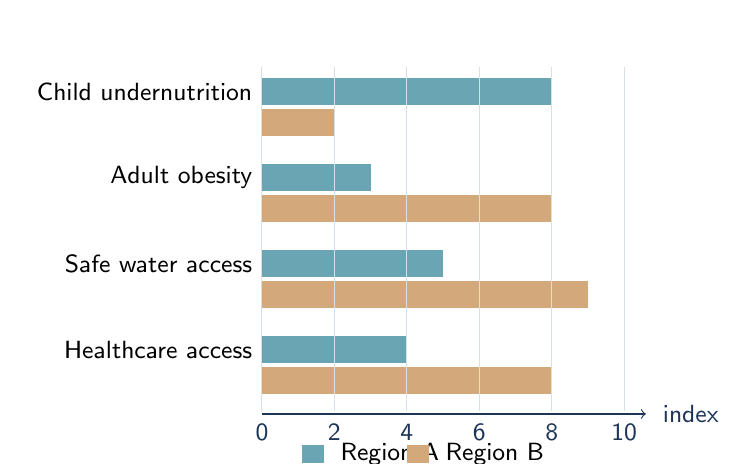
\begin{tikzpicture}[x=0.46cm,y=0.78cm, every node/.style={font=\sffamily\small}]
  \node[anchor=east] at (0,5.4) {Child undernutrition};
  \draw[fill=AccentTeal!70, draw=none] (0,5.18) rectangle (8,5.62);
  \draw[fill=AccentGold!75, draw=none] (0,4.68) rectangle (2,5.12);

  \node[anchor=east] at (0,4.0) {Adult obesity};
  \draw[fill=AccentTeal!70, draw=none] (0,3.78) rectangle (3,4.22);
  \draw[fill=AccentGold!75, draw=none] (0,3.28) rectangle (8,3.72);

  \node[anchor=east] at (0,2.6) {Safe water access};
  \draw[fill=AccentTeal!70, draw=none] (0,2.38) rectangle (5,2.82);
  \draw[fill=AccentGold!75, draw=none] (0,1.88) rectangle (9,2.32);

  \node[anchor=east] at (0,1.2) {Healthcare access};
  \draw[fill=AccentTeal!70, draw=none] (0,0.98) rectangle (4,1.42);
  \draw[fill=AccentGold!75, draw=none] (0,0.48) rectangle (8,0.92);

  \foreach \x in {0,2,4,6,8,10} {
    \draw[RuleGray] (\x,0.2) -- (\x,5.8);
    \node[below, color=HeadingBlue] at (\x,0.15) {\x};
  }
  \draw[->, color=HeadingBlue] (0,0.15) -- (10.6,0.15);
  \node[anchor=west, color=HeadingBlue] at (10.8,0.15) {index};

  \draw[fill=AccentTeal!70, draw=none] (1.1,-0.65) rectangle (1.7,-0.35);
  \node[anchor=west] at (1.9,-0.5) {Region A};
  \draw[fill=AccentGold!75, draw=none] (4.0,-0.65) rectangle (4.6,-0.35);
  \node[anchor=west] at (4.8,-0.5) {Region B};
\end{tikzpicture}
\end{center}

\textbf{Timed prompt.} Using Source A, write \term{4--5} short-response points
describing and explaining the pattern of food and health inequality between
Region A and Region B.

\subsection{Source B: Resource Security Map}

The map below is a simplified practice map of four districts in one river
basin. The labels show the main resource-security pressure in each district.

\begin{center}
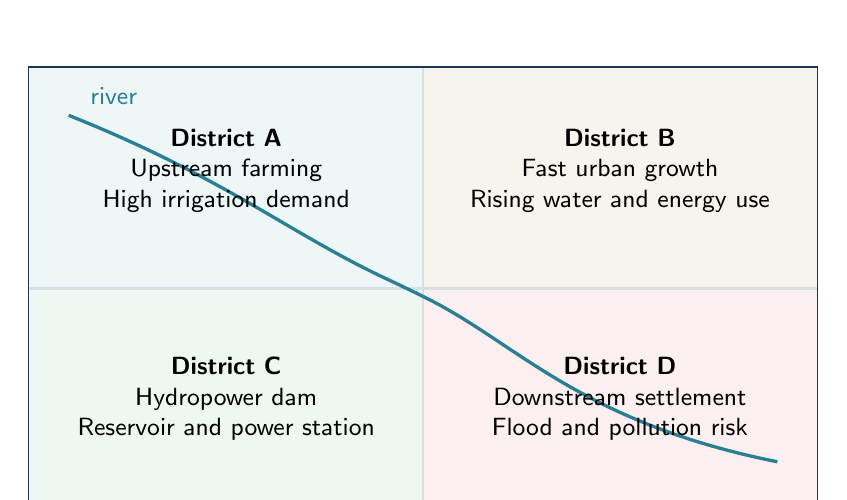
\begin{tikzpicture}[every node/.style={font=\sffamily\small}]
  \draw[very thick, color=HeadingBlue] (0,0) rectangle (10,5.6);
  \fill[SoftBlue] (0,2.8) rectangle (5,5.6);
  \fill[SoftTint] (5,2.8) rectangle (10,5.6);
  \fill[SoftGreen] (0,0) rectangle (5,2.8);
  \fill[SoftRed] (5,0) rectangle (10,2.8);

  \draw[RuleGray, thick] (5,0) -- (5,5.6);
  \draw[RuleGray, thick] (0,2.8) -- (10,2.8);
  \draw[AccentTeal, very thick, rounded corners=8pt] (0.5,5.0) .. controls
  (2.5,4.2) and (3.3,3.5) .. (4.8,2.8) .. controls (6.2,2.1) and
  (7.0,1.1) .. (9.5,0.6);

  \node[align=center, text width=4cm] at (2.5,4.3)
  {\textbf{District A}\\Upstream farming\\High irrigation demand};
  \node[align=center, text width=4cm] at (7.5,4.3)
  {\textbf{District B}\\Fast urban growth\\Rising water and energy use};
  \node[align=center, text width=4cm] at (2.5,1.4)
  {\textbf{District C}\\Hydropower dam\\Reservoir and power station};
  \node[align=center, text width=4cm] at (7.5,1.4)
  {\textbf{District D}\\Downstream settlement\\Flood and pollution risk};

  \node[anchor=west, color=AccentTeal] at (0.65,5.25) {river};
\end{tikzpicture}
\end{center}

\textbf{Timed prompt.} Using Source B, write \term{4--5} short-response points
explaining how resource-security pressures vary within the river basin.

\subsection{Source C: E-Waste Flow Table}

The table below is illustrative practice evidence for a resource-consumption
and waste-management question.

\rowcolors{2}{TableStripe}{white}
\begin{tabularx}{\textwidth}{L{0.22\textwidth}Y Y}
\toprule
\textbf{Stage} & \textbf{Linear pattern} & \textbf{Circular-economy alternative} \\
\midrule
Purchase & Frequent device replacement and high material demand & Longer use,
repair, leasing, shared devices, and right-to-repair policies \\
Use & Energy use and rapid obsolescence & Efficient devices, software support,
and durable design \\
Disposal & Export, landfill, informal processing, or low-value recycling & Safe
collection, producer responsibility, certified recycling, and material recovery \\
Impact & Pollution, worker health risk, lost metals, and pressure shifted to
other places & Lower extraction pressure, less pollution, local jobs, but higher
cost and governance needs \\
\bottomrule
\end{tabularx}
\rowcolors{2}{}{}

\textbf{Timed prompt.} Using Source C, write \term{4--5} short-response points
explaining why e-waste is a resource-security and environmental-management
issue.

\section{Response Space}

\subsection{Source Chosen}

Circle one: \term{A Food and health graph} \quad \term{B Resource map} \quad
\term{C E-waste table}

\subsection{4--5 Short-Response Points}

Use complete sentences. Each point should include evidence, course vocabulary,
and a consequence or explanation.

\begin{enumerate}
  \item \blankbox{white}{1.55cm}
  \item \blankbox{white}{1.55cm}
  \item \blankbox{white}{1.55cm}
  \item \blankbox{white}{1.55cm}
  \item \blankbox{white}{1.55cm}
\end{enumerate}

\section{Self-Mark Guide}

\rowcolors{2}{TableStripe}{white}
\begin{tabularx}{\textwidth}{L{0.14\textwidth}Y Y}
\toprule
\textbf{Point} & \textbf{Credit if it includes...} & \textbf{Fix if missing...} \\
\midrule
1 & Overall trend or pattern from the source & Add a sentence beginning
"Overall..." \\
2 & Specific highest, lowest, or most affected category/place & Name the
category or district and quote the visible evidence \\
3 & Comparison between two places, groups, or stages & Use "whereas",
"compared with", or "in contrast" \\
4 & Explanation using course vocabulary such as food access, disease diffusion,
resource security, nexus, or circular economy & Add "because" and a process
word \\
5 & Impact, implication, limitation, or management response & Add "this matters
because..." \\
\bottomrule
\end{tabularx}
\rowcolors{2}{}{}

\subsection{Possible Strong Points}

Use these only after your timed attempt.

\begin{itemize}
  \item \textbf{Source A:} Region A shows higher child undernutrition while
  Region B shows higher adult obesity, suggesting different food-health
  problems rather than one simple measure of "healthy" or "unhealthy."
  \item \textbf{Source A:} Region B's higher safe-water and healthcare access
  may reduce infectious disease risk, but high obesity suggests nutrition
  transition or processed-food access may create non-communicable disease risk.
  \item \textbf{Source B:} The river basin shows a water-energy-food nexus:
  upstream irrigation, urban demand, hydropower, and downstream pollution or
  flood risk affect one another.
  \item \textbf{Source B:} District C may improve energy security through
  hydropower, but it creates trade-offs for ecosystems, downstream flow, and
  possibly communities.
  \item \textbf{Source C:} E-waste is a resource issue because discarded devices
  contain recoverable materials; poor disposal loses resources and may shift
  pollution risks to other places.
  \item \textbf{Source C:} Circular-economy approaches can reduce extraction
  and pollution, but they depend on regulation, collection systems, producer
  responsibility, and consumer behavior.
\end{itemize}

\section{Error Log}

\begin{tabularx}{\textwidth}{L{0.27\textwidth}Y}
\toprule
\textbf{Question} & \textbf{My answer} \\
\midrule
Did I quote visible evidence? & \smallline \\[0.8em]
Did I compare two places, groups, or stages? & \smallline \\[0.8em]
Did I explain using course vocabulary? & \smallline \\[0.8em]
Did I add an impact or management implication? & \smallline \\[0.8em]
One thing to improve tomorrow & \smallline \\[0.8em]
\bottomrule
\end{tabularx}

\section{Case-Study Watchlist}

These are not required for today's timed visual-data task, but they should be
filled on the May 1 case-study bank day.

\begin{tabularx}{\textwidth}{L{0.28\textwidth}Y}
\toprule
\textbf{Gap} & \textbf{What to add before the exam} \\
\midrule
Food and health disease case & Named disease, place, transmission route,
vulnerable group, response, and one limitation \\[0.6em]
Resources stewardship case & Named place or policy, resource issue, management
response, impact, and one trade-off or limitation \\[0.6em]
\bottomrule
\end{tabularx}

\section{Exit Ticket}

Before closing the workbook, write one sentence for each chain.

\begin{tabularx}{\textwidth}{L{0.28\textwidth}Y}
\toprule
\textbf{Chain} & \textbf{Sentence} \\
\midrule
Food system $\rightarrow$ health & \smallline \\[1.1em]
Disease condition $\rightarrow$ spread & \smallline \\[1.1em]
Consumption $\rightarrow$ resource security & \smallline \\[1.1em]
Nexus trade-off & \smallline \\[1.1em]
\bottomrule
\end{tabularx}

\end{document}
